\subsection{Verfahren zum Verwenden maximaler Batchgrößen}
\todo[inline]{Über Lars schreiben; 3 Stunden}
Zum Training eines CNN werden die Daten in der Regel in Batches aufgeteilt. Übliche Trainingsverfahren verwenden dabei eine Batchgröße, die nur einen Bruchteil des verfügbaren Grafikspeichers belegt. Dies geschieht, da mit einer maximalen Batchgröße weniger Aktualisierungen der Gewichte pro Trainingsepoche vorgenommen werden. So entsteht beim Training mit maximaler Batchgröße eine verminderte Generalisierungsfähigkeit. Das Ergebnis eines CNNs abhängig von der Batchgröße wird anhand eines Beispieldatensatzes in Abbildung \ref{abb:largeB1} gezeigt. Es ist zu beobachten, dass circa ab Epoche 85 eine Rangfolge von hoher Batchgröße hin zu niedriger Batchgröße in Bezug auf die Accuracy erreicht wird. Diese Rangfolge ändert sich auch bis zum Ende des Trainings nicht mehr. 


\begin{figure}[h]
 \centering
 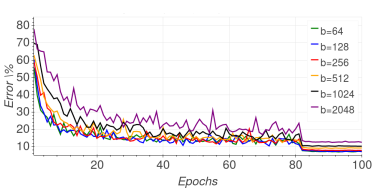
\includegraphics[width=0.8\textwidth]{KapitelPartA/images/batchSize1.png}
 % batchSize1.png: 383x191 px, 72dpi, 13.51x6.74 cm, bb=0 0 383 191
 \caption{Validation Accuracy von CNNs anhand eines Beispieldatensatzes}
 \label{abb:largeB1}
\end{figure}


Die Quelle zu diesem Kapitel untersucht dieses Problem und schlägt eine Lösung vor \cite{lars}.
Für das Training mit kleinen Batchgrößen wird im Allgemeinen ein Stochastisches Gradientenabstiegsverfahren (SGD) benutzt. 


Large Batch (ghost batch norm) hat leider nicht funktioniert. Dem Paper scheinen wichtige Detail s zu fehlen.

Eine alternative ist Lars. (LARGE BATCH TRAINING OF CONVOLUTIONAL NET -
WORKS WITH LAYER - WISE A DAPTIVE R ATE S CALING)

Dabei wird keine globale Lernrate mehr verwendet, sondern die Lernrate wird an die Größe der Gewichte angepasst. 

Funktioniert nach einem ersten auch zusammen mit Prune Train um bei größerer Batchgröße weiterhin trotzdem eine gute Verkleinerungsrate zu bekommen.
\color{black}
